\documentclass[11pt,letterpaper]{article}
\usepackage{fullpage}

\usepackage[english]{babel}
\usepackage[utf8]{inputenc}
\usepackage{amsmath}
\usepackage{graphicx}
\usepackage[hidelinks]{hyperref}
\usepackage{float}
\usepackage{amsfonts}
\usepackage{algorithm,algpseudocode}
\usepackage{pdfpages}
             
\graphicspath{{../results}}

\begin{document} 

\title{New Experiments}
\maketitle

\section*{Vary Warm Start + Effective end of game}

Here we vary the size of the warm start (the number of observations given to the principals before the competing bandits game begins). We also track a new quantity - the ``effective end of game" which we define as the last round where there is a ``switch" in the decision of the agent. So, for instance, if in $t-1$ the agent picks principal 1 and in $t$ the agent picks principal 2 then this is a ``switch." The last time this happens in a simulation is defined as effective end of game (EEOG).

Below we report the results of running on the same priors we have been considering, but varying the warm start and recording market share + EEOG.
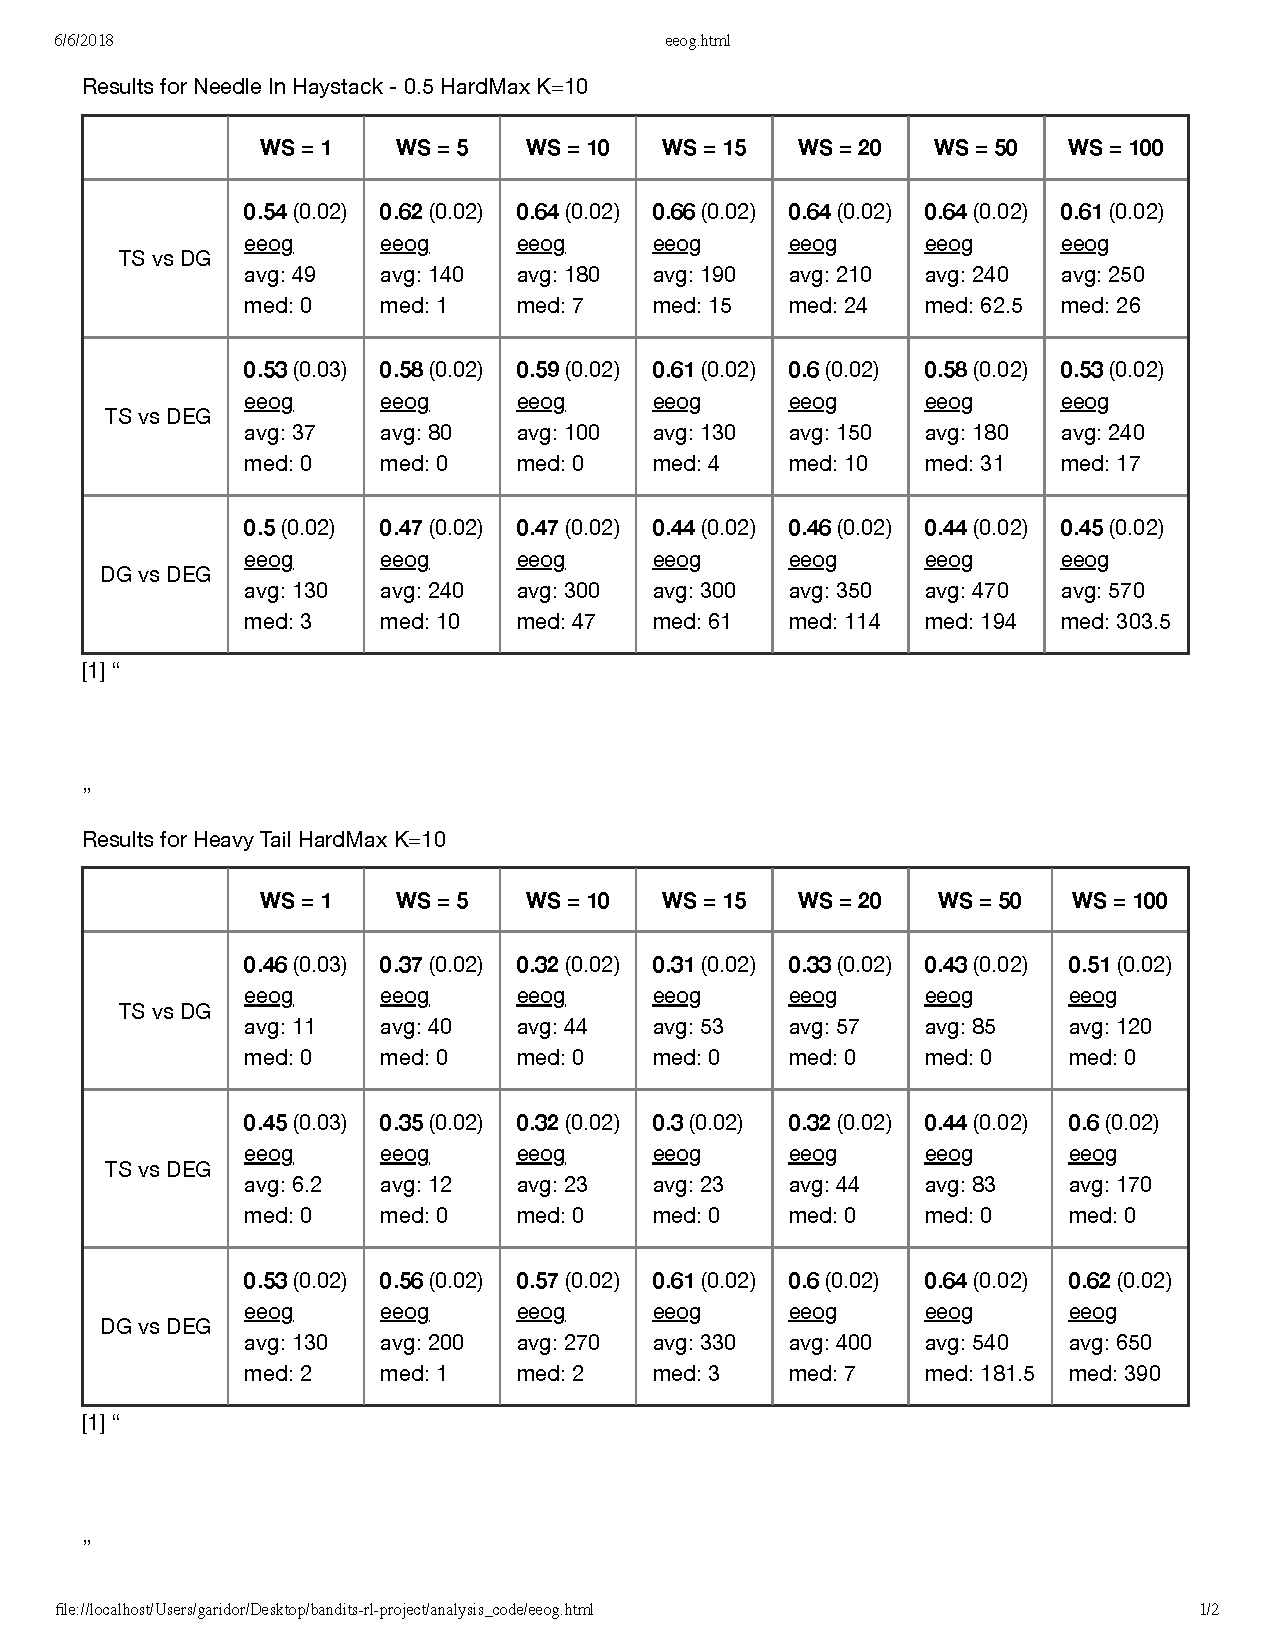
\includepdf[pages={-}]{eeog_old_priors}

\section*{.5/.7 Instance}

This is an instance where the arms are uniformly either 0.5 or 0.7 (as opposed to Needle in a Haystack where 9 arms have mean 0.5 and 1 arm has mean 0.7).

This is what the preliminary calibration for this instance looks like:

\includegraphics[scale=0.5]{"Reputation Trajectory for 5_7"}

The results of the simulations:

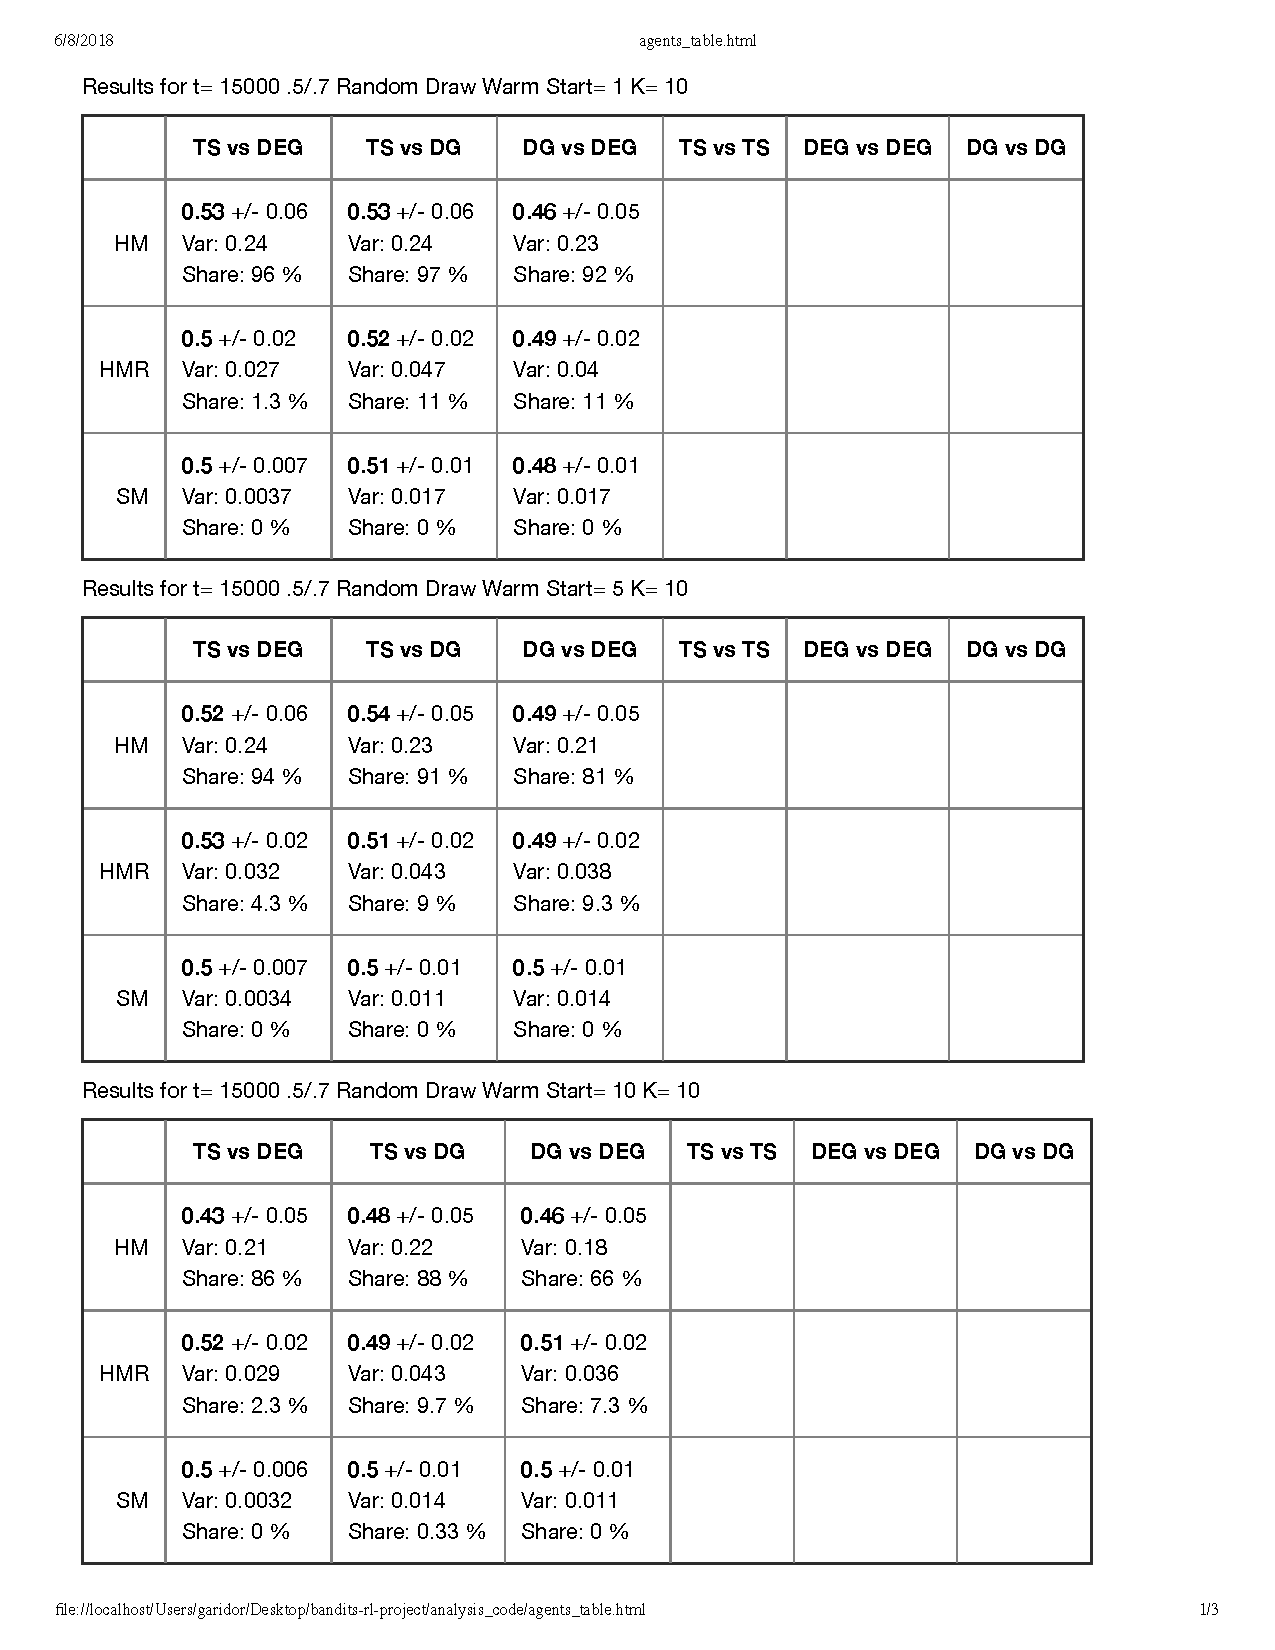
\includepdf[pages={-}]{5_7_results}


\section*{Various Needles in a Haystack}
In this set of experiments we simply shift the needle in a haystack distribution.

We consider the following instances:
\begin{enumerate}
\item Needle In Haystack 0.1 - 9 arms with mean 0.1, 1 arm with mean 0.3
\item Needle In Haystack 0.3 - 9 arms with mean 0.3, 1 arm with mean 0.5
\item Needle In Haystack 0.5 - 9 arms with mean 0.5, 1 arm with mean 0.7
\item Needle In Haystack 0.7 - 9 arms with mean 0.5, 1 arm with mean 0.7
\end{enumerate}


Preliminary plots for 0.1 and 0.3: \\
\includegraphics[scale=0.4]{"./Reputation Trajectory for Needle In Haystack 1 10 arms"} \\
\includegraphics[scale=0.4]{"./Reputation Trajectory for Needle In Haystack 3 10 arms"}

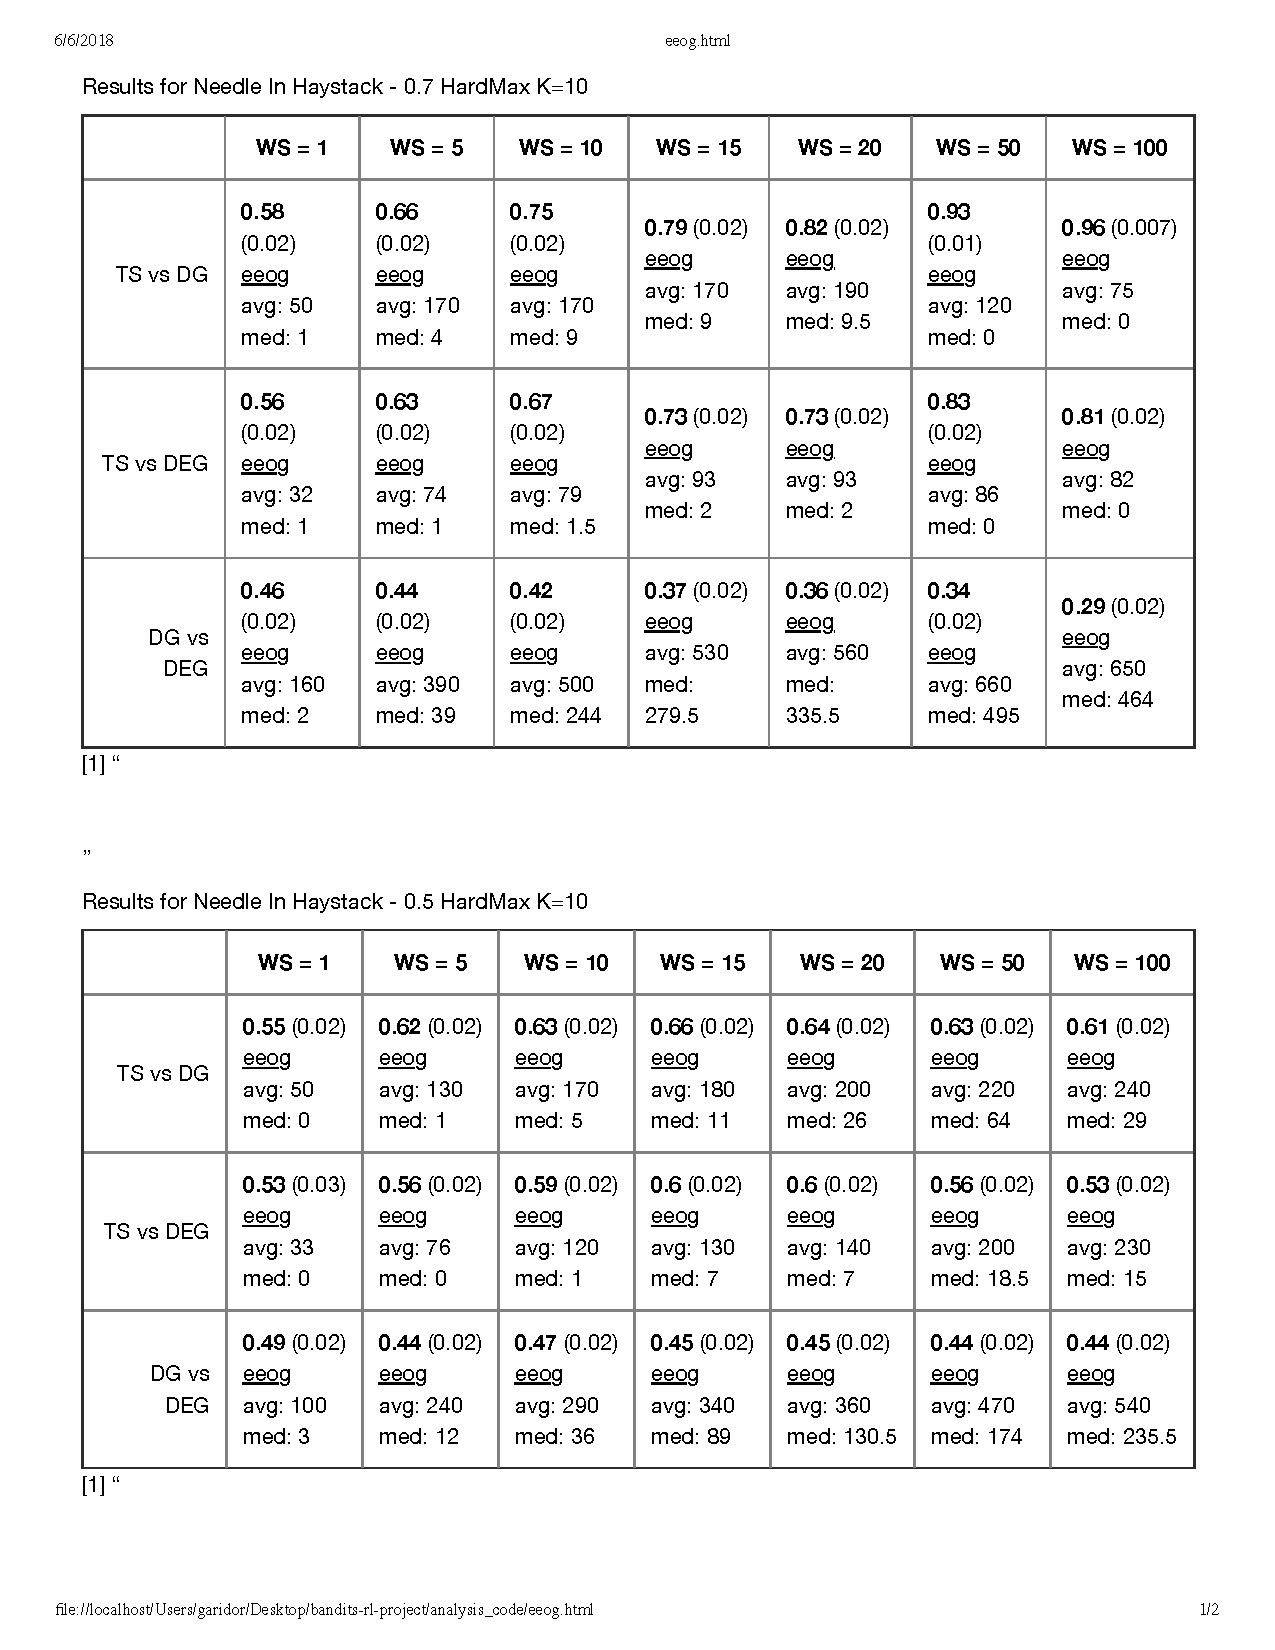
\includepdf[pages={-}]{haystack_eeog}



\end{document}
